\chapter{Related Work}
%Summary: 2 major sections, 1 about past radio instrumentation, 1 about automatic mapping\\
%Goal: Explain why we can mesh them together successfully in this case\\
%State: Can be written now \\
%List of references already compiled into Papers archive \\
\section{Radio Astronomy} \label{Related Work:Radio Astronomy}
%\subsection{Digital Signal Processing for Radio Astronomy}
\subsection{DiFX}

\begin{figure}[ht!]
  \centering
    \includegraphics[width=\textwidth]{Images/C3/difx_architecture.pdf}
  \caption{TODO}
  \label{fig: C3/difx_architecture.pdf}
\end{figure}

%TODO: If you have a cluster available�
%Why do cpu-only?
%It�s easy
%Compared to 27 antenna 2GHz EVLA in New Mexico
The DiFX Correlator is a scalable software implementation of an FX Correlator  \cite{Deller:2007wy}.
The correlator was originally developed to do VLBI (Very Long Baseline interfereometery). 
DiFX was designed as a software correlator in order to maintain flexibility in the design, but that flexibility comes at a high hardware cost. 
To process 64 MHz of bandwidth and only 10 antennas, about 100 nodes are required to cross correlate all the data. 
%TODO: define expensive

%DiFX (Distributed FX Correlator) is a scalable software implementation
%Designed for VLBI (Very Long Baseline Interferometry)
%Requires a large cluster to do a lot of computation
%64 MHz, 10 antennas required ~100 nodes in 2007

\subsection{LOFAR}
\begin{figure}[ht!]
  \centering
    \includegraphics[width=\textwidth]{Images/C3/lofar_performance.pdf}
  \caption{TODO Lofar Performance}
  \label{fig: C3/lofar_performance.pdf}
\end{figure}
%On a blue gene, real time but still costly power hungry solution 64 stations
%TODO: read this paper
Like DiFX, the correlator for Low-Frequency Array for Radio Astronomy (or LOFAR) was also built using CPUs \cite{vanNieuwpoort:2009p1253}.
This project used a Blue Gene BG/P %TODO: check this
to implement a 64 station correlator.
The implementation got very high performance out of the cluster, 96\% of the peak, but required an entire cluster and required finely tuned code to achieve that performance. 


\subsection{xGPU}
%TODO: add another graph from paper
\begin{figure}[ht!]
  \centering
    \includegraphics[width=\textwidth]{Images/C3/gpuxperformance.pdf}
  \caption{TODO}
  \label{fig: C3/gpuxperformance.pdf}
\end{figure}

\cite{Clark:2011wi}

\cite{2009PASP..121..857W}


\subsection{CASPER}
%TODO: work this in
The need for high bandwidth spectroscopy manifests in many different radio astronomy applications.
Keeping up with increasing computation demands has often resulted in the specialized design of spectrometers.
At the Collaboration for Astronomy Signal Processing and Electronics Research (CASPER), we have developed a software package to automatically generate spectrometers for a variety of applications.

\begin{figure}[ht!]
  \centering
    \includegraphics[width=\textwidth]{Images/C3/casper_collaborators.png}
  \caption{TODO}
  \label{fig: C3/casper_collaborators.png}
\end{figure}

The CASPER FPGA libraries were developed to mitigate the need to redevelop common signal processing blocks for every new instrument \cite{Parsons:2006cu}. 
Parameterized blocks such as FFTs and digital down-converters can easily be used to design many different instruments. 
Coupled with open source FPGA boards, such as the ROACH (Reconfigurable Open Architecture Computing Hardware), the CASPER libraries provide a useful toolbox for radio astronomy instrumentation development.


The goal of Collaboration for Astronomy Signal Processing and Electronics Research (CASPER) is to provide common libraries, tools, and hardware for radio astronomers developing instrumentation. 

\subsubsection{CASPER Hardware}

The CASPER group provides set of modular FPGA boards and ADCs that are designed specifically to deal with the high bandwidth requirements of real time radio astronomy signal processing. 
Since these boards are designed for the needs of the radio astronomy community as a whole rather than a single application, the group provides a small set of powerful boards. 
The boards can be upgraded one by one, or all at once since they communicate over a common set of industry standard protocols and use a standard signal processing model. 
The CASPER library and software, discussed below, also make it easy to upgrade the hardware since a CASPER design easily be recompiled to work with a different board and the software interface and the signal processing model are standardized.

Each FPGA board implements a number of high speed interfaces to send and receive data.
The Z-DOK+ connectors are primarily used to interface the boards to high speed ADCs and DACs.
This common Z-DOK+ interconnect allows the astronomer to choose an ADC to match their scientific goals. 


\begin{table}
\begin{tabular}{| l | l | l | l |}
\hline  
\textbf{ADC Name} & Max sample rate & Streams & Bitwidth \\
\hline  
64ADCx64-12 & 50 Msps & 64 & 12 bits\\
ADC4x250-8 or QuadADC & 250 Msps & 4 & 8 bits\\
KatADC & 1.5 Gsps & 1 & 8 bits  \\
ADC1X2200-10 & 2.2 Gsps & 1 & 10 bits \\
ADC1x10000-4 & 10 Gsps & 1 & 4 bits \\
\hline  
\end{tabular}
\end{table} 


%TODO: finish this 
%Boards work with a variety of ADCs/DACs etc.
%Dual input 8 bit 1 Gsps (or 2 Gsps single input interleaved)
%3 Gsps single input 8 bit ADC (interleave 2 for 6 Gsps)
%Provides tested hardware for new instruments

Each board also send or receive data using ethernet. 
The boards are designed to communicate using common protocols, like 10GbE, so a board can be upgraded without modifying how it communicates with other boards. 
The use of 10GbE also makes communication to non-CASPER boards simple, allowing an FPGA to create UDP packets that eventually get processed on a CPU or GPU server, making these boards an ideal component of a heterogeneous cluster. 
This makes it simple to design a cluster, and allows continuous upgrades as technology improves, as the signal processing model and communication model do not change between boards.


%All boards can talk to each other
%Can�t clock FPGA at 3GHz but use parallel FFT 8-16 samples at a time
%BEE2 lib w/Bob Broderson

%TODO: add roach 2, bee2, ibob
\begin{figure}[ht!]
  \centering
    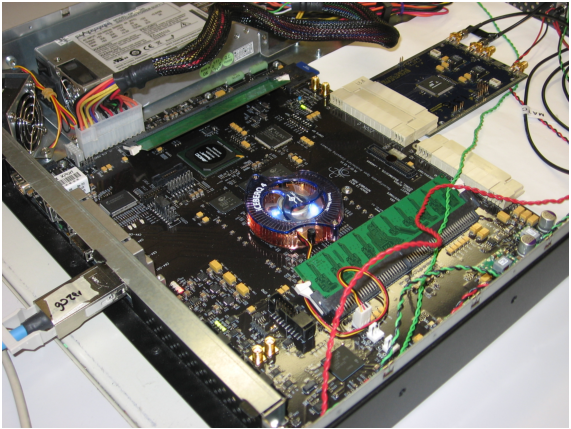
\includegraphics[width=\textwidth]{Images/C3/roach.pdf}
  \caption{TODO ROACH}
  \label{fig: C3/roach.pdf}
\end{figure}

The ROACH board, shown in Figure \ref{fig: C3/roach.pdf}, with an iADC board connected via Z-DOK+ and an ethernet cable to get data off the board. 




\subsubsection{CASPER Library}

%  Platform independent DSP library
%  Blocks can be used on any CASPER board (BEE2 or iBOB,
%ROACH coming soon...)
%  Currently restricted to Xilinx chips but can be ported to other platforms
%  Large set of parameterizable DSP building blocks
%  FFTs (tunable bandwidth, number of channels, real or complex) ?  PFBs
%  Accumulators
%  All library blocks are built from Xilinx primitive blocks
%  Matlab scripts (�mask scripts�) are used to configure parameterized blocks

%TODO: edit this
In addition to hardware, CASPER also develops a Simulink library designed for real time radio astronomy signal processing.
These boards are designed to provide high bandwidth I/O and dense computation.
CASPER seeks to develop a small number of boards that can be deployed without a lot of effort and upgraded without doing a major redesign of the instrument. 
The Simulink designs can be retargeted to different boards without changed the original implementation.
The library is implemented in Simulink, which allows for both simulation and, using Xilinx System Generator, compilation to FPGA code.

%CASPER = Collaboration for Astronomy Signal Processing and Electronics Research
%Identifies commonly used DSP blocks for radio astronomy
%FFTs (tunable bandwidth, number of channels, real or complex)
%Polyphase filter banks
%Accumulators
%Digital downconverters/mixers
%Scripts are used to configure parameterized blocks

\begin{figure}
  \centering
     \includegraphics[width=\textwidth]{Images/C3/casper_fft_lib.pdf}
  \caption{TODO}
  \label{fig:casper_fft_lib.pdf}
\end{figure}

This is achieved by identifying commonly used DSP blocks in radio astronomy instruments and developing parameterized implementations of these common blocks, making them useful for a variety of instruments. 
For example, the CASPER library provides FFTs, polyphase filter banks, accumulators, digital downconverters, digital mixers which can be linked together to make an instrument. 
Figure \ref{fig:casper_fft_lib.pdf} shows the FFT library, which contains different types of FFTs, including blocks that can process multiple samples in parallel and blocks that are optimized to compute the FFT of a real signal. 


\begin{figure}
  \centering
     \includegraphics[width=0.45\textwidth]{Images/C3/casper_fft_lib_options.pdf}
  \caption{TODO}
  \label{fig:casper_fft_lib_options.pdf}
\end{figure}


Figure \ref{fig:casper_fft_lib_options.pdf} shows the options menu for one of the FFT blocks. 
In order to support a variety of instruments, the block can be reconfigured to support different FFT lengths.
There are a number of other parameters provided like input bit width, which helps support a number of different ADCs or preprocessing algorithms, and FPGA-specific parameters like add latency, and multiply latency which have no effect on the result of the computation but change how the FFT gets mapped into hardware. 

\begin{figure}[ht!]
  \centering
    \includegraphics[width=0.49\textwidth]{Images/C3/adder_tree_diagram.pdf}
    \includegraphics[width=0.49\textwidth]{Images/C3/adder_tree_code.pdf}
  \caption{TODO}
  \label{fig: C3/adder_tree}
\end{figure}


These parameters in the options menu are implemented using a number of matlab scripts to automatically design the block. 



%TODO: maybe break this down into separate blocks
\begin{figure}
  \centering
     \includegraphics[width=0.75\textwidth]{Images/C3/yellow_blocks.pdf}
  \caption{TODO}
  \label{fig:yellow_blocks.pdf}
\end{figure}

The CASPER library also provides a set of blocks to abstract away the implementation of I/O interfaces, which are called yellow blocks. 
Figure \ref{fig:yellow_blocks.pdf} provides some examples of what those library blocks look like. 
Each block provides input and output ports that correspond to the data it can send or receive. 
For example, the adc block has an output port that represents the data coming from the iADC and is received by the board.
In addition to this, simulation ports are provided to allow the user to proved test signals mimicking the outside world.
In the case of the adc, the user could provide a sine wave into the \emph{sim\_in} port to observe how a sine wave would be processed by the system.
During compilation, the CASPER XPS toolflow automatically processes the blocks and ensures the interfaces are implemented correctly in the final bitfile.



\subsubsection{CASPER Software}

%Toolflow for compilation, ref BEE2 compile path, borph, etc
%TODO: add reference-BORPH
To simplify the use of the FPGA further, the CASPER boards run a modified version of linux directly on the board. 
Using this linux environment, called the Berkeley Os for ReProgrammable Hardware or BORPH, programming the FPGA is as simple as running an executable on the command line. \cite{So:2007ve}
Then, once the board has been programmed, BORPH can communicate with the chip using a interface where components on the FPGA like registers or memory appear as a file system in the operating system. 
These files can be accessed using normal file I/O, making it simple to send control signals or monitor the status of the chip.

\cite{Cross:2009ta}

\subsubsection{SERENDIP V.v}

\begin{figure}[ht!]
  \centering
    \includegraphics[width=\textwidth]{Images/C3/setispectrometerv55.pdf}
  \caption{TODO}
  \label{fig: C3/setispectrometerv55.pdf}
\end{figure}

%Used for the SETI ALFA Survey, JPL Sky Survey, and Argentina SETI
%  200 MHz Bandwidth currently, future plans to upgrade to 300MHz
%  128 Million frequency channels
%  Build using an iADC, iBOB and BEE2
%  Can process one polarization from a single beam

\begin{figure}[ht!]
  \centering
    \includegraphics[width=\textwidth]{Images/C3/alfa_feed.png}
  \caption{TODO}
  \label{fig: C3/alfa_feed.png}
\end{figure}

\begin{figure}[ht!]
  \centering
    \includegraphics[width=0.48\textwidth]{Images/C3/serendip_vv_top.png}
    \includegraphics[width=0.48\textwidth]{Images/C3/serendip_vv_bottom.png}
  \caption{TODO}
  \label{fig: C3/serendipvv}
\end{figure}

%4k point PFB
%  32k by 4k corner turn
%  32k point FFT
%  Each element (PFB, corner turn, FFT, and thresholder) is on a separate BEE2 chip
%  Output to PC is low bandwidth due to thresholding
%  Upcoming ROACH architecture will support 2 polarizations, 400 MHz

%SuccessfullydeployedatAreciboObservatoryinJune2009
%  ImplementedonanIBOBandBEE2board
%  200MHzbandwidth
%  28million(227)channels(4kcoarsechannels*32kfinechannels)
%  1. 5 Hz/channel
%  0. 67 sec integration time
%  ObservescommensallywithallALFAobservations
%  Observesonlyonebeamatatime

%Arecibo L-band Feed Array
%?  7 pixel dual polarization ?  ALFA RF 1225-1525 MHz

\cite{2010LPICo1538.5378S}


\subsubsection{CASPER Correlator}
\begin{figure}[ht!]
  \centering
    \includegraphics[width=\textwidth]{Images/C3/casper_correlator.png}
  \caption{TODO}
  \label{fig: C3/casper_correlator.png}
\end{figure}

\cite{Parsons:2008dl}

%Used to develop Parsons/Manley correlator
%10GbE switch solves cabling problem
%Still have N^2 X engines

\section{Tuning} \label{Related Work:Tuning}
\subsection{Metropolis}

The Metropolis project focused on mapping algorithms onto embedded system \cite{Davare:2007ue}. 
The tool provides a framework for an abstract block based description of an embedded system. 
This description makes it easy to stitch algorithms together without specifying the eventual hardware implementation, providing a simple path to simulation and algorithm development that is separate from the implemented design. 
Then, the tool automatically maps the description onto an existing heterogeneous embedded system. 

%TODO: review references
\cite{Balarin:2003kc}
\cite{Densmore:tm}

%Mapping is focused on scheduling onto heterogeneous platforms
%Strong focus on embedded systems

%Some people have thought about how to use technology
%Metropolis works on simulation extensively (supporting 
%Embedded systems � we have 1 cpu and 1 dsp let�s make it go fast
%This doesn�t solve our problem
%Just does scheduling

The mapping generated by the tool is simply a schedule, specifying where and when each part of the computation gets executed. 
The tool seeks to optimize performance of the algorithm, ensuring the generated schedule runs as fast as possible on the hardware provided. 
This technique requires a fixed hardware model and uses the existing hardware to optimize performance. 
While this work is useful when a hardware model exists, it does not provide any flexibility in the hardware model while mapping the algorithm. 
So, when it is necessary to design the hardware to begin with, this does not solve the problem. 

%Doesn�t help design the cluster
%A �heterogeneous node� has a fixed mix of resources
%Can�t reduce costs by throwing away certain types of hardware
%Optimization is based on a fixed architecture and flexible performance
%Doesn�t match our �always running� model
%Performance is �good enough�, not an optimization target

Additionally, this type of solution is ill-suited to mapping the computation required to do real-time radio astronomy signal processing. 
This tool assumes it must schedule a discrete task onto a fixed piece of hardware and attempts maximize the performance of the task. 
In the applications described in Chapter \ref{chap:Real Time Radio Astronomy Algorithms}, the computation should always be running and needs to meet some minimum performance target.
Once the performance target is met, it's better to have a tool that will other costs like power or amount of hardware, rather attempting to improve the runtime of the algorithm. 








%Lisa Marie Guerra (?)


\subsection{ILP for scheduling}
An integer linear programming model for mapping applications on hybrid systems

%TODO: sort these out
\cite{Gibeling:2008vg}

\cite{Theodoridis:2009gd}

\cite{Tsoi:2010we}

\cite{Jun:2008vv}

\cite{Rakhshanfar:2011tg}